\documentclass[11pt]{article}
\usepackage{geometry,marginnote} % Pour passer au format A4
\geometry{hmargin=1cm, vmargin=1cm} % 

% Page et encodage
\usepackage[T1]{fontenc} % Use 8-bit encoding that has 256 glyphs
\usepackage[english,french]{babel} % Français et anglais
\usepackage[utf8]{inputenc} 

\usepackage{lmodern,numprint}
\setlength\parindent{0pt}

% Graphiques
\usepackage{graphicx,float,grffile,units}
\usepackage{tikz,pst-eucl,pst-plot,pstricks,pst-node,pstricks-add,pst-fun,pgfplots} 

% Maths et divers
\usepackage{amsmath,amsfonts,amssymb,amsthm,verbatim}
\usepackage{multicol,enumitem,url,eurosym,gensymb,tabularx}

\DeclareUnicodeCharacter{20AC}{\euro}



% Sections
\usepackage{sectsty} % Allows customizing section commands
\allsectionsfont{\centering \normalfont\scshape}

% Tête et pied de page
\usepackage{fancyhdr} \pagestyle{fancyplain} \fancyhead{} \fancyfoot{}

\renewcommand{\headrulewidth}{0pt} % Remove header underlines
\renewcommand{\footrulewidth}{0pt} % Remove footer underlines

\newcommand{\horrule}[1]{\rule{\linewidth}{#1}} % Create horizontal rule command with 1 argument of height

\newcommand{\Pointilles}[1][3]{%
  \multido{}{#1}{\makebox[\linewidth]{\dotfill}\\[\parskip]
}}

\newtheorem{Definition}{Définition}

\usepackage{siunitx}
\sisetup{
    detect-all,
    output-decimal-marker={,},
    group-minimum-digits = 3,
    group-separator={~},
    number-unit-separator={~},
    inter-unit-product={~}
}

\setlength{\columnseprule}{1pt}

\begin{document}

\textbf{Nom, Prénom :} \hspace{8cm} \textbf{Classe :} \hspace{3cm} \textbf{Date :}\\

\begin{center}
  \textit{La plus coûteuse des dépenses, c’est la perte de temps.}  - \textbf{Théophraste}
\end{center}

\subsection*{Restituer les connaissances}

\begin{enumerate}
  \item[1.] Définition : Triangle. \newline \Pointilles[1]
  \item[2.] Propriété : Angles. \newline \Pointilles[1]
  \item[3.] Propriété : Inégalité triangulaire. \newline \Pointilles[1]
\end{enumerate}

\subsection*{ex1 - Calculer les angles dans les triangles}
\textbf{(modéliser, écrire le calcul, calculer)}

\begin{figure}[H]
  \centering
  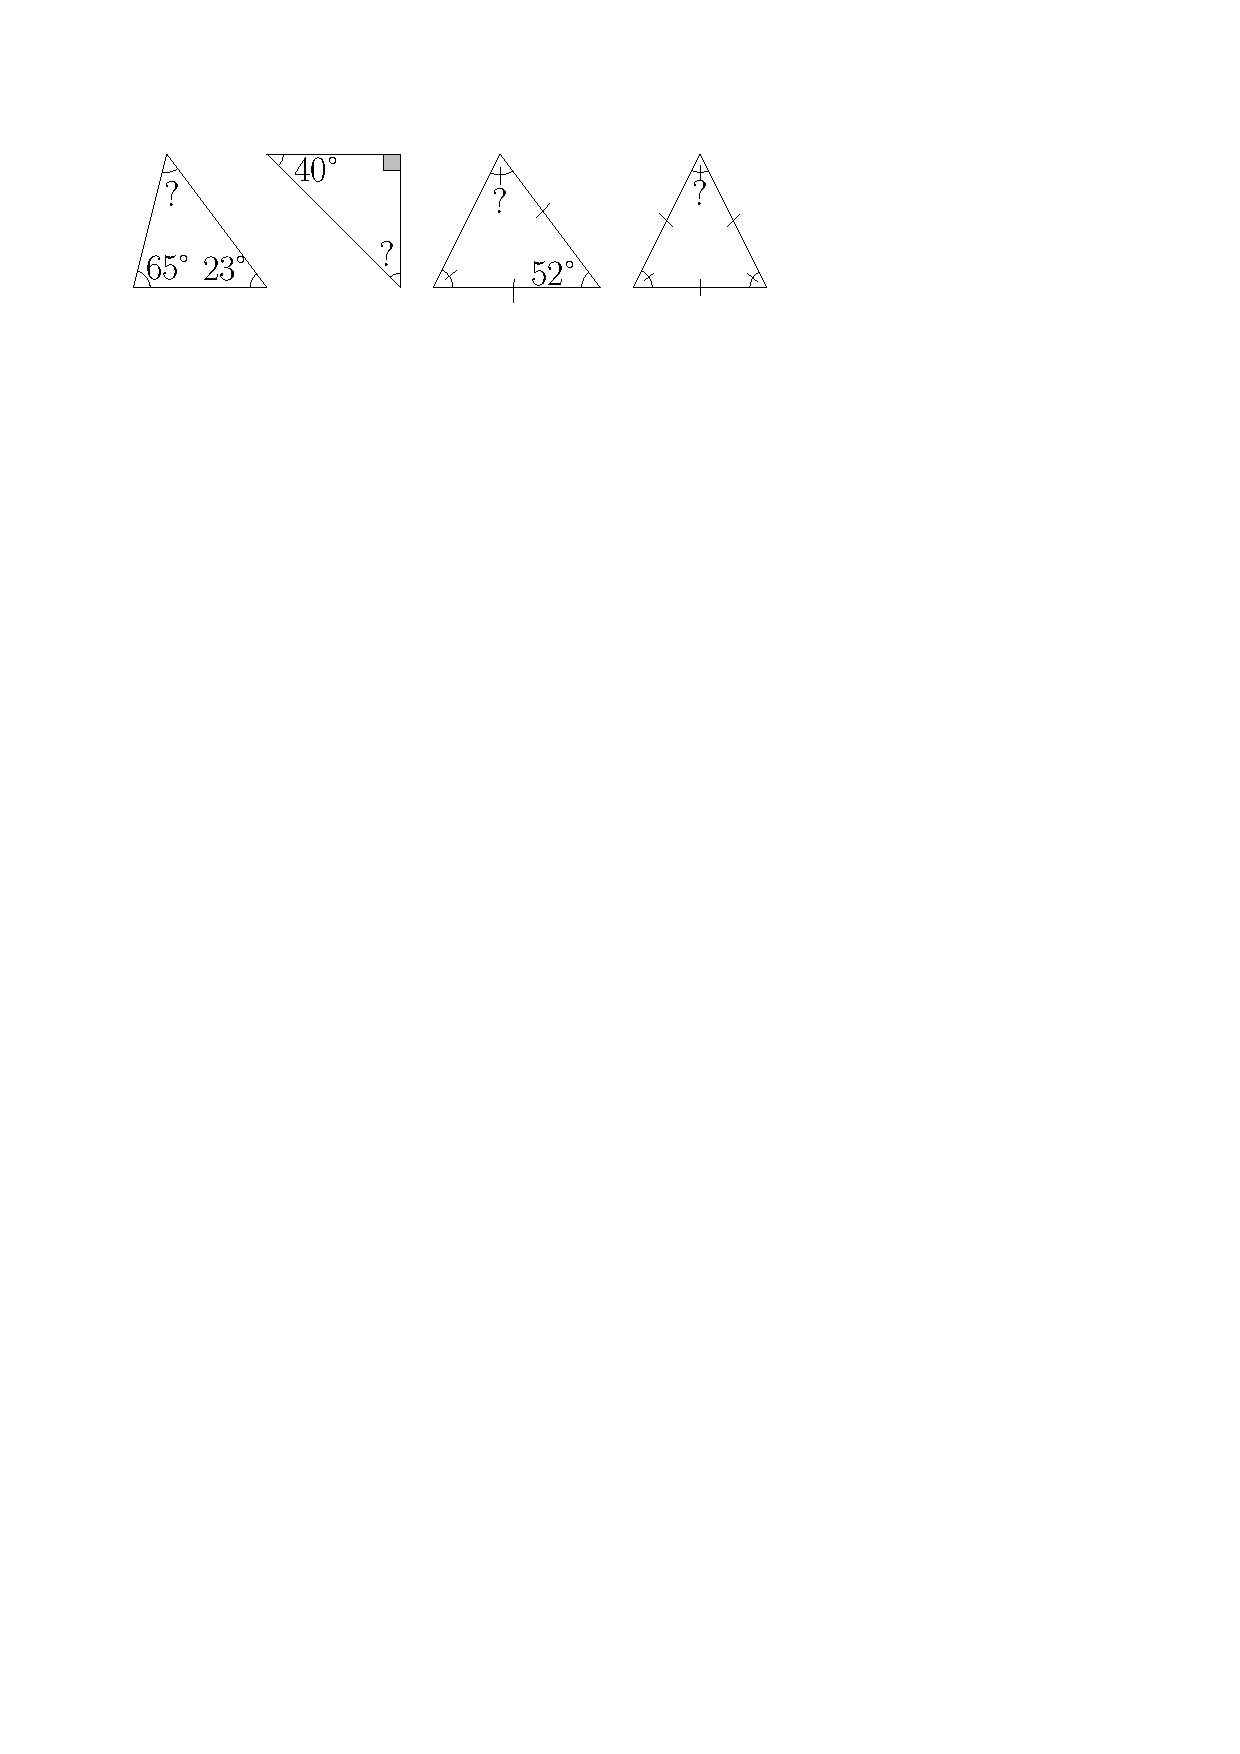
\includegraphics[width=0.55\linewidth]{5x3-triangles/ie-ex1a.pdf}
\end{figure}

\begin{multicols}{4}
\Pointilles[3] 
\columnbreak 

\Pointilles[3] 
\columnbreak 

\Pointilles[3] 
\columnbreak 

\Pointilles[3] 
\columnbreak 
\end{multicols}


\subsection*{ex3 - Démontrer}
\textit{Peut-on tracer les triangles suivants ?}
\textbf{(justifier, écrire les calculs, conclure)}

\begin{enumerate}
  \item[1.] Peut-on tracer le triangle AVC tel que : AV = 12cm ; AC = 6cm et VC = 4cm ? 
  \item[2.] Peut-on tracer le triangle PLS tel que : PL = 200m ; LS = 305m et PS = 150m ? 
  \item[3.] Peut-on tracer le triangle UMP tel que : UM = 30cm ; MP = 5m et UP = 34cm ?  
\end{enumerate} 

\Pointilles[14] 


\newpage

\subsection*{ex2 - Calculer les angles}
\textbf{(justifier, modéliser, écrire les calculs, calculer)}

\begin{minipage}[t]{0.4\textwidth}
  \begin{figure}[H]
    \centering
    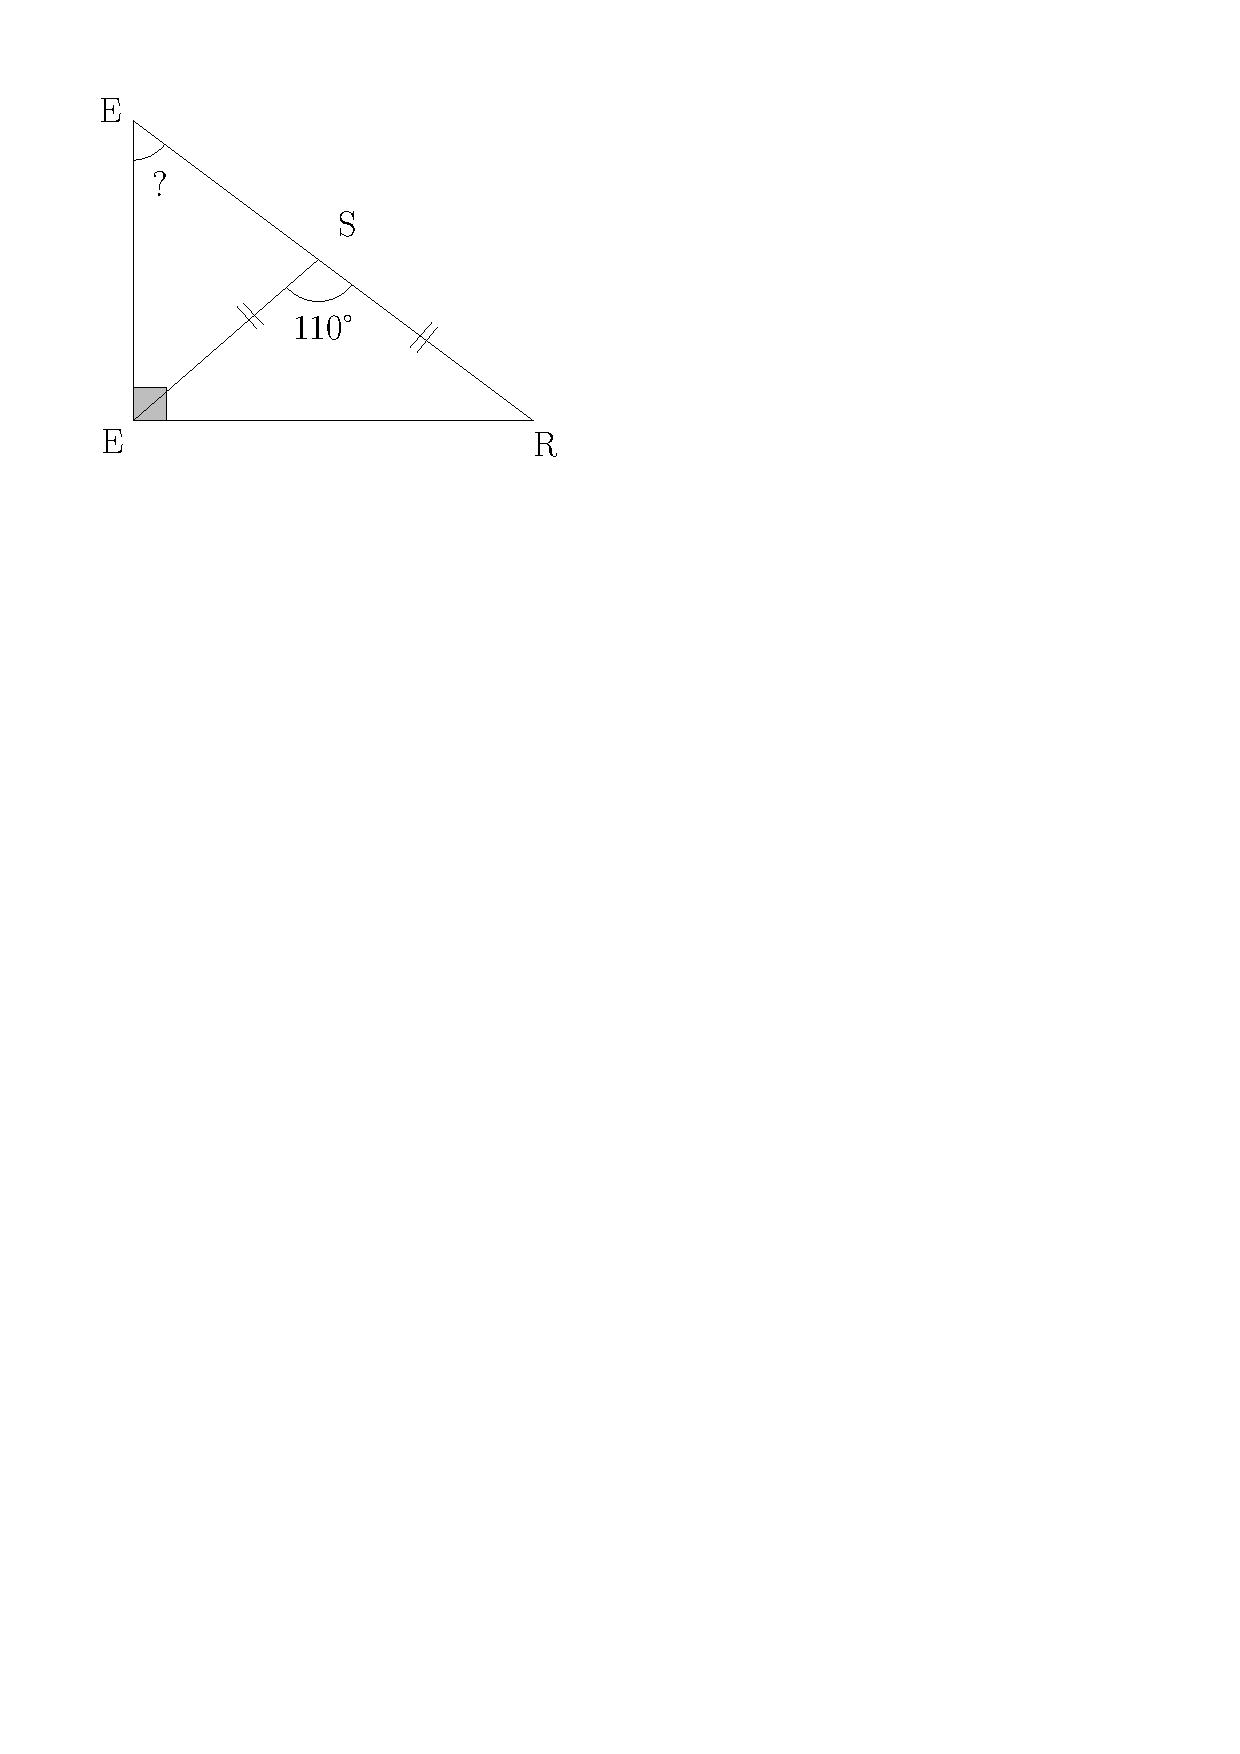
\includegraphics[width=0.6\linewidth]{5x3-triangles/ie-ex2a1.pdf}
  \end{figure}

\end{minipage}
\begin{minipage}[t]{0.6\textwidth}

  \Pointilles[8] \\
\end{minipage}

\begin{minipage}[t]{0.4\textwidth}
  \begin{figure}[H]
    \centering
    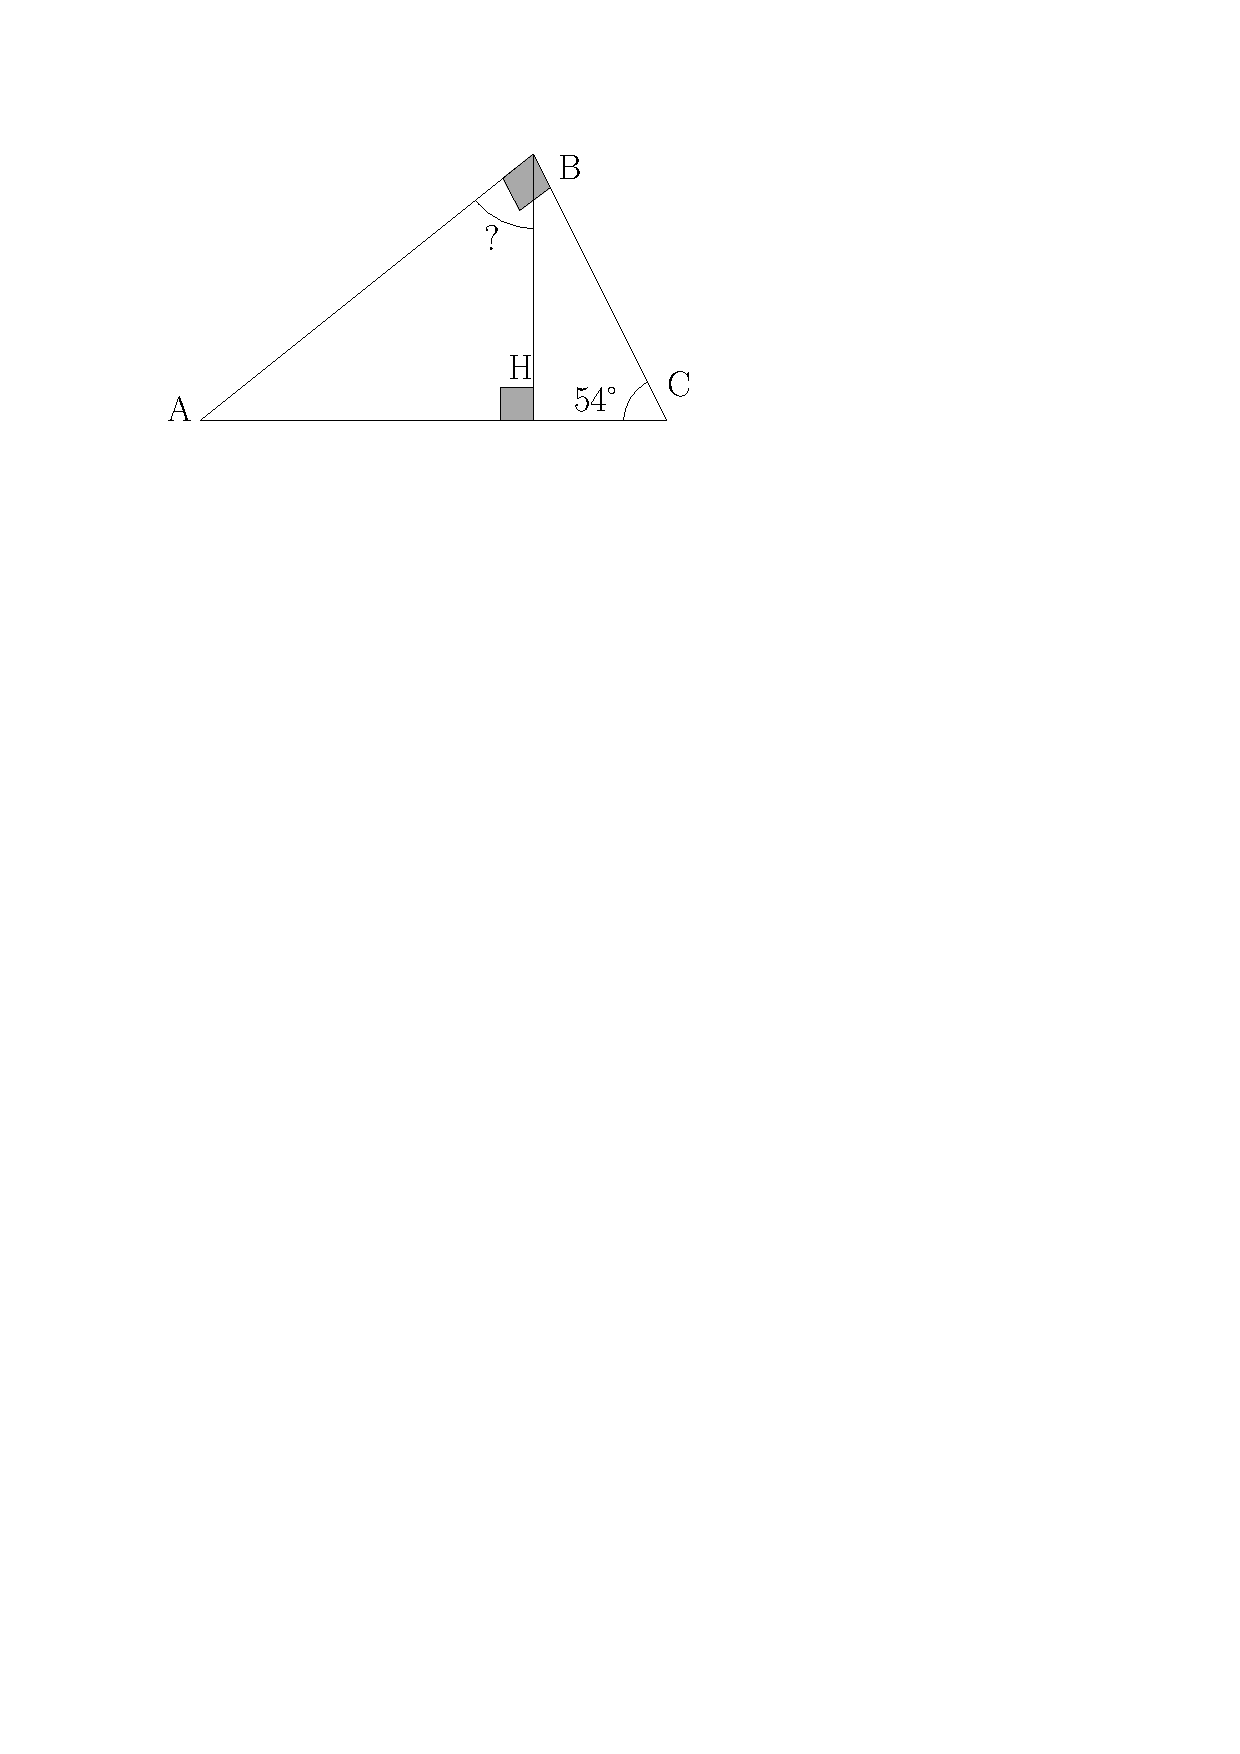
\includegraphics[width=0.8\linewidth]{5x3-triangles/ie-ex2b1.pdf}
  \end{figure} 

\end{minipage}
\begin{minipage}[t]{0.6\textwidth}

  \Pointilles[8] \\
\end{minipage}

\begin{minipage}[t]{0.4\textwidth}
\begin{figure}[H]
    \centering
    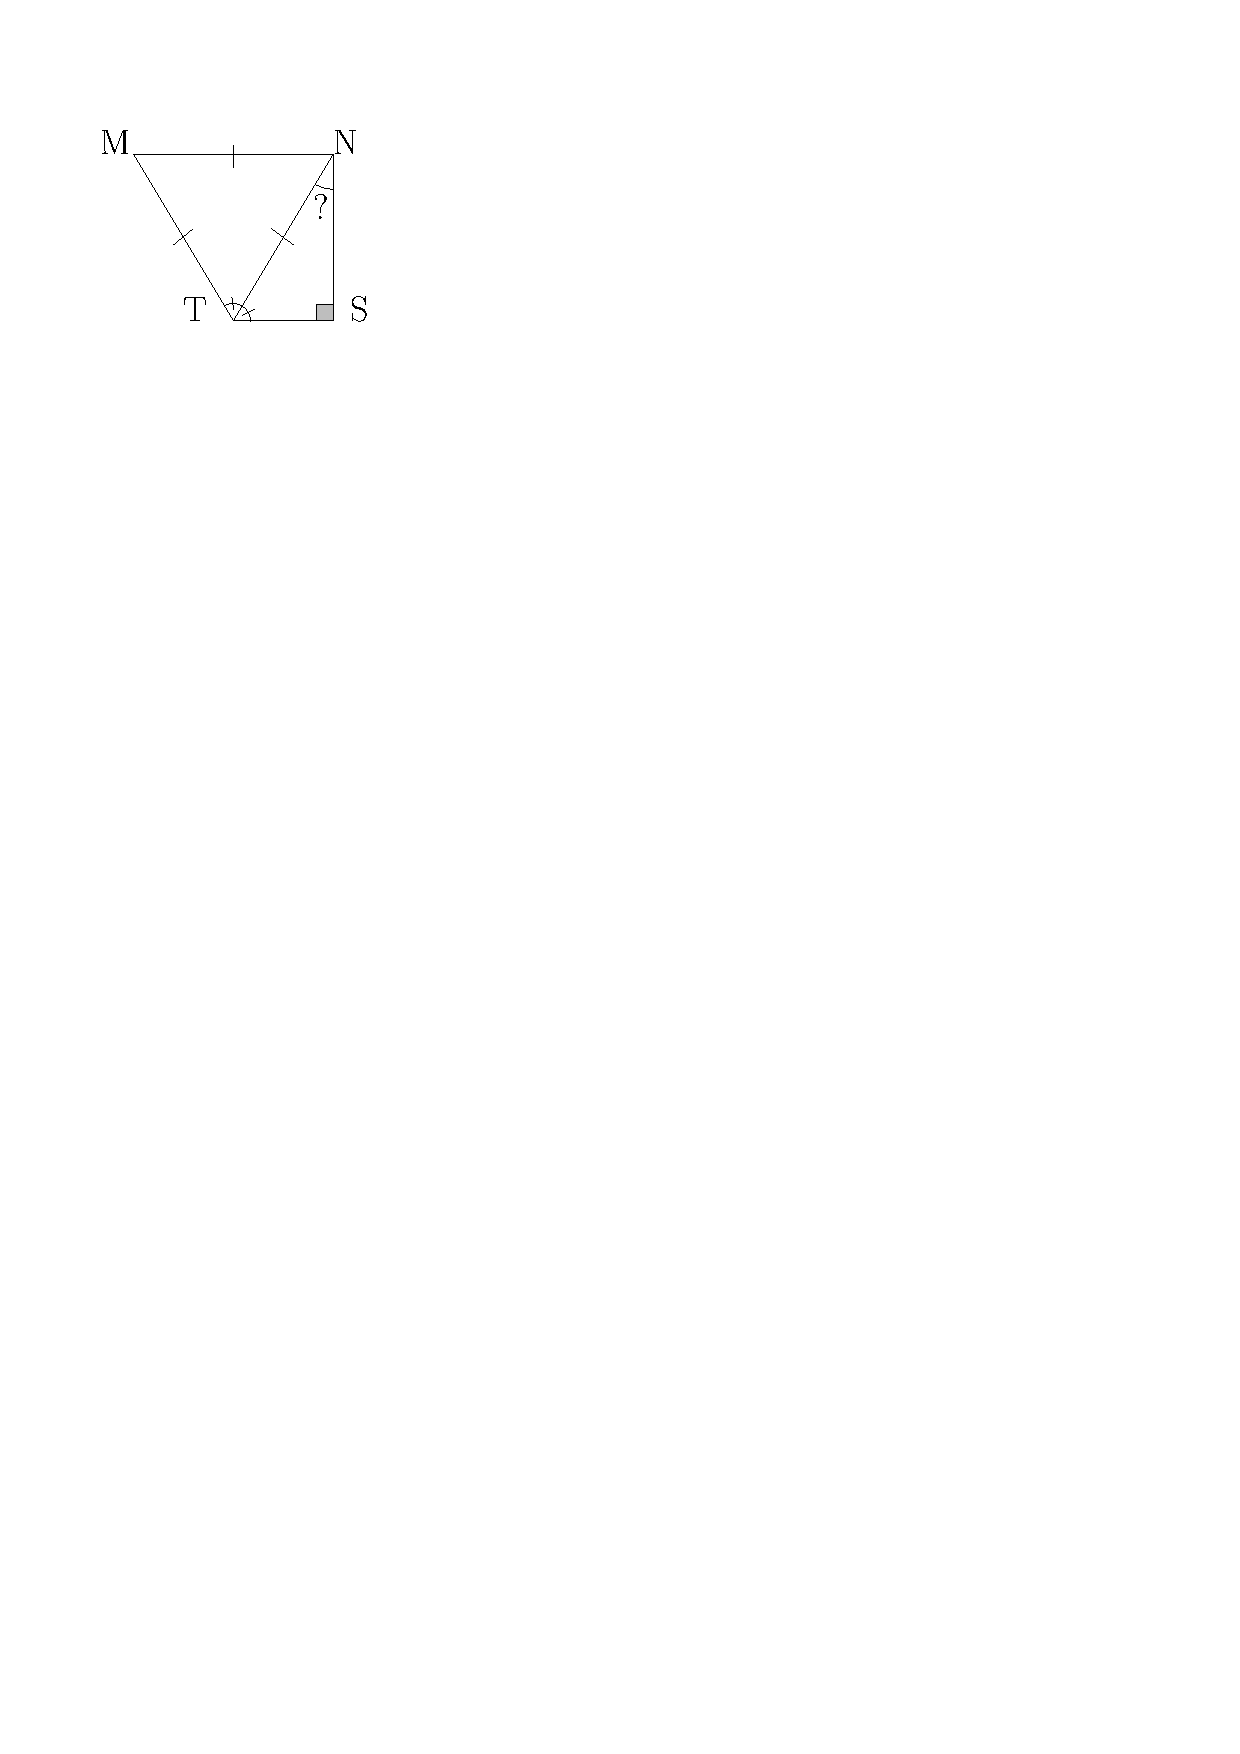
\includegraphics[width=0.6\linewidth]{5x3-triangles/ie-ex2c.pdf}
  \end{figure} 

\end{minipage}
\begin{minipage}[t]{0.6\textwidth}

  \Pointilles[8]
\end{minipage}



\subsection*{ex3 - Démontrer}

\begin{enumerate}
  \item[1.] \textbf{(aucune justification n'est demandée.)}

    Jean-mi veut construire un triangle ABC dont il connaît les longueurs AB et AC. \newline
    Parmi les longueurs proposées pour BC, \textbf{entourer la ou les mesures possibles}.

    \begin{multicols}{2}
      \begin{tabular}{|c|c||c|c|c|}
        \hline
          AB & AC & BC & BC & BC\\ \hline
          34 & 18 & 10 & 20 & 30\\ \hline
           4 & 10 & 10 & 20 & 30\\ \hline
          12 & 21 & 10 & 20 & 30\\ \hline
       $\pi$ &  7 & 10 & 20 & 30\\ \hline
      \end{tabular}
      
      \columnbreak

      \textit{(les pointillés peuvent servir de brouillon)}
      \Pointilles[4]
    \end{multicols}

  \item[2.] \textbf{(justifier, calculer, conclure.)}
  
  Soit ARN un triangle tel que AR = 15 cm et RN = 5 cm. \newline
  \textbf{Quelles sont les mesures entières possibles pour AN ?}

  \Pointilles[6]
\end{enumerate} 

\newpage

\textbf{Nom, Prénom :} \hspace{8cm} \textbf{Classe :} \hspace{3cm} \textbf{Date :}\\

\begin{center}
  \textit{La plus coûteuse des dépenses, c’est la perte de temps.}  - \textbf{Théophraste}
\end{center}

\subsection*{Restituer les connaissances}

\begin{enumerate}
  \item[1.] Définition : Triangle. \newline \Pointilles[1]
  \item[2.] Propriété : Angles. \newline \Pointilles[1]
  \item[3.] Propriété : Inégalité triangulaire. \newline \Pointilles[1]
\end{enumerate}

\subsection*{ex1 - Calculer les angles dans les triangles}
\textbf{(modéliser, écrire le calcul, calculer)}

\begin{figure}[H]
  \centering
  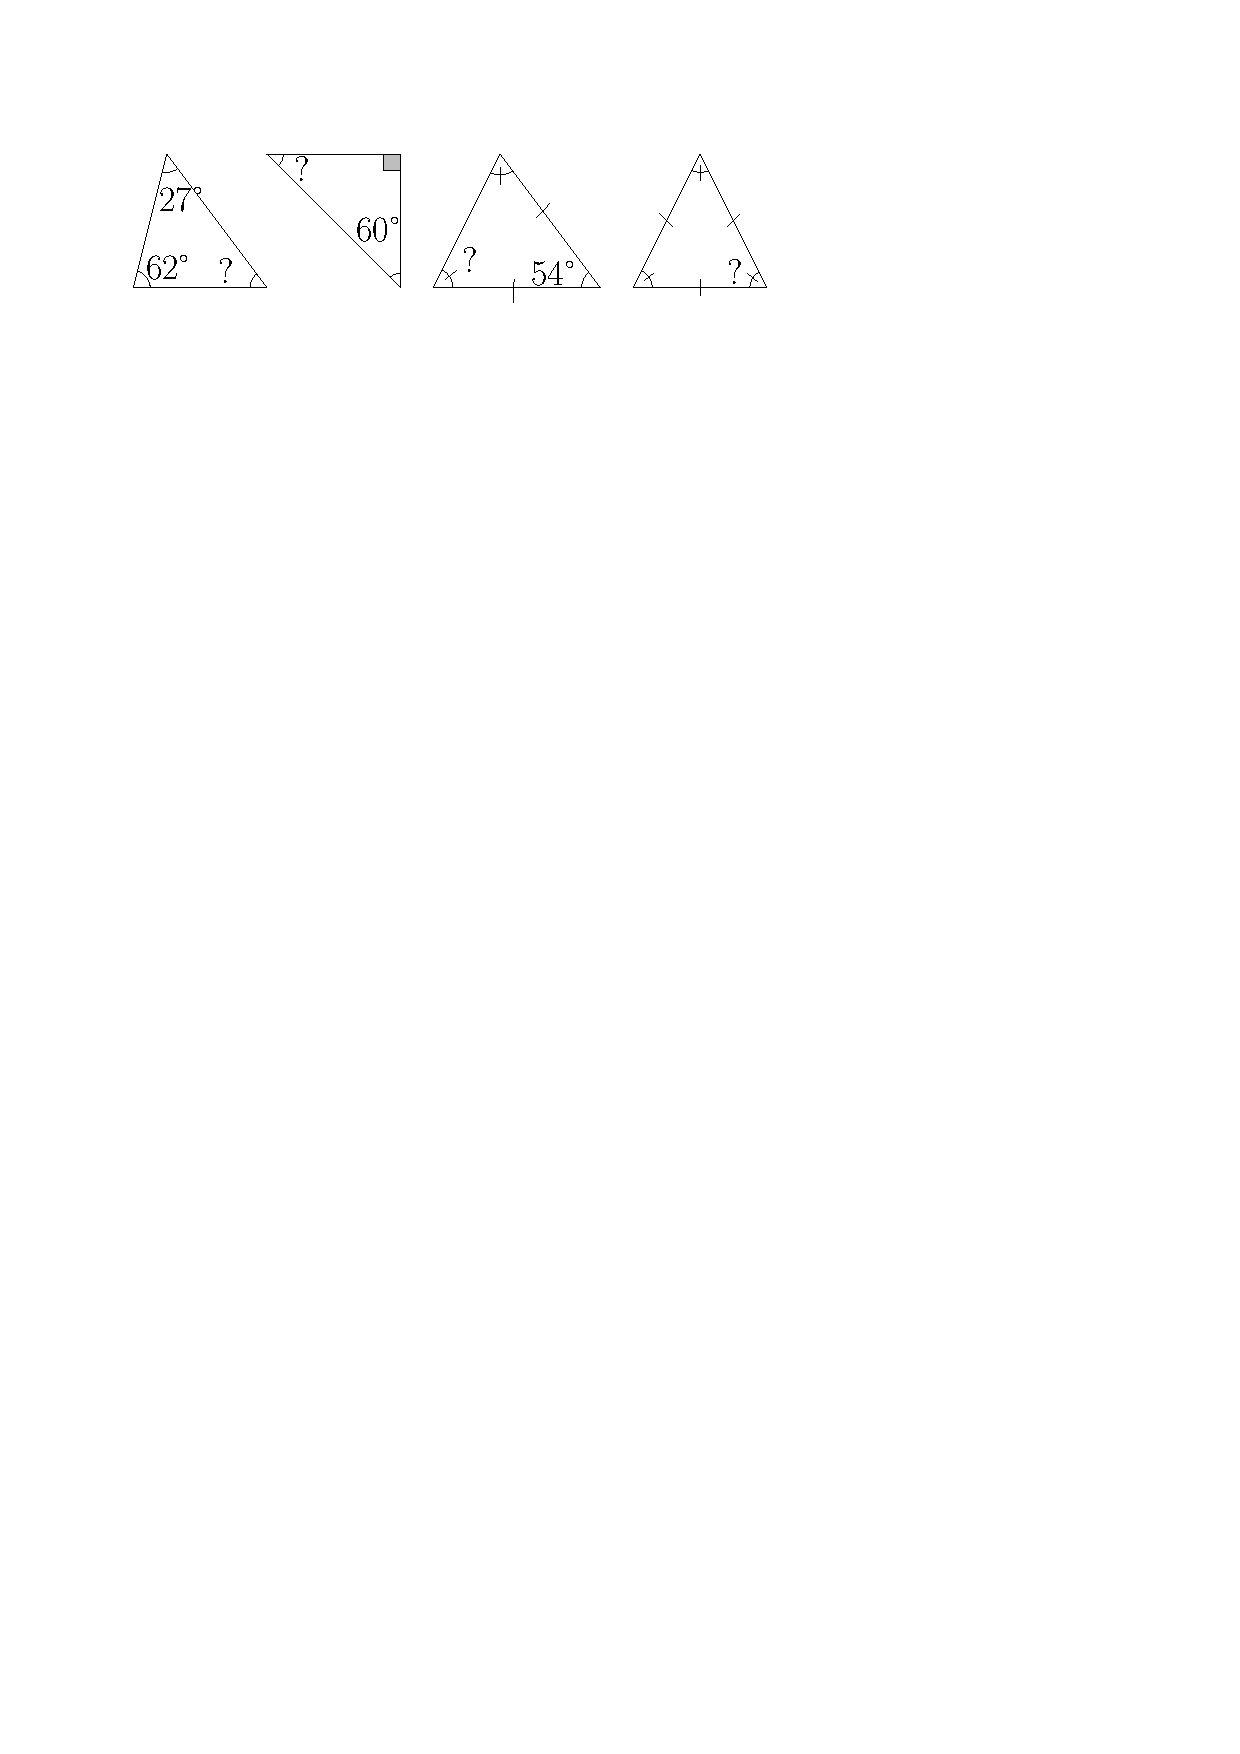
\includegraphics[width=0.55\linewidth]{5x3-triangles/ie-ex1b.pdf}
\end{figure}

\begin{multicols}{4}
\Pointilles[3] 
\columnbreak 

\Pointilles[3] 
\columnbreak 

\Pointilles[3] 
\columnbreak 

\Pointilles[3] 
\columnbreak 
\end{multicols}


\subsection*{ex3 - Démontrer}
\textit{Peut-on tracer les triangles suivants ?}
\textbf{(justifier, écrire les calculs, conclure)}

\begin{enumerate}
  \item[1.] Peut-on tracer le triangle AVC tel que : AV = 22cm ; AC = 16cm et VC = 4cm ? 
  \item[2.] Peut-on tracer le triangle PLS tel que : PL = 300m ; LS = 405m et PS = 150m ? 
  \item[3.] Peut-on tracer le triangle UMP tel que : UM = 20cm ; MP = 5m et UP = 24cm ?  
\end{enumerate} 

\Pointilles[14] 


\newpage

\subsection*{ex2 - Calculer les angles}
\textbf{(justifier, modéliser, écrire les calculs, calculer)}

\begin{minipage}[t]{0.4\textwidth}
  \begin{figure}[H]
    \centering
    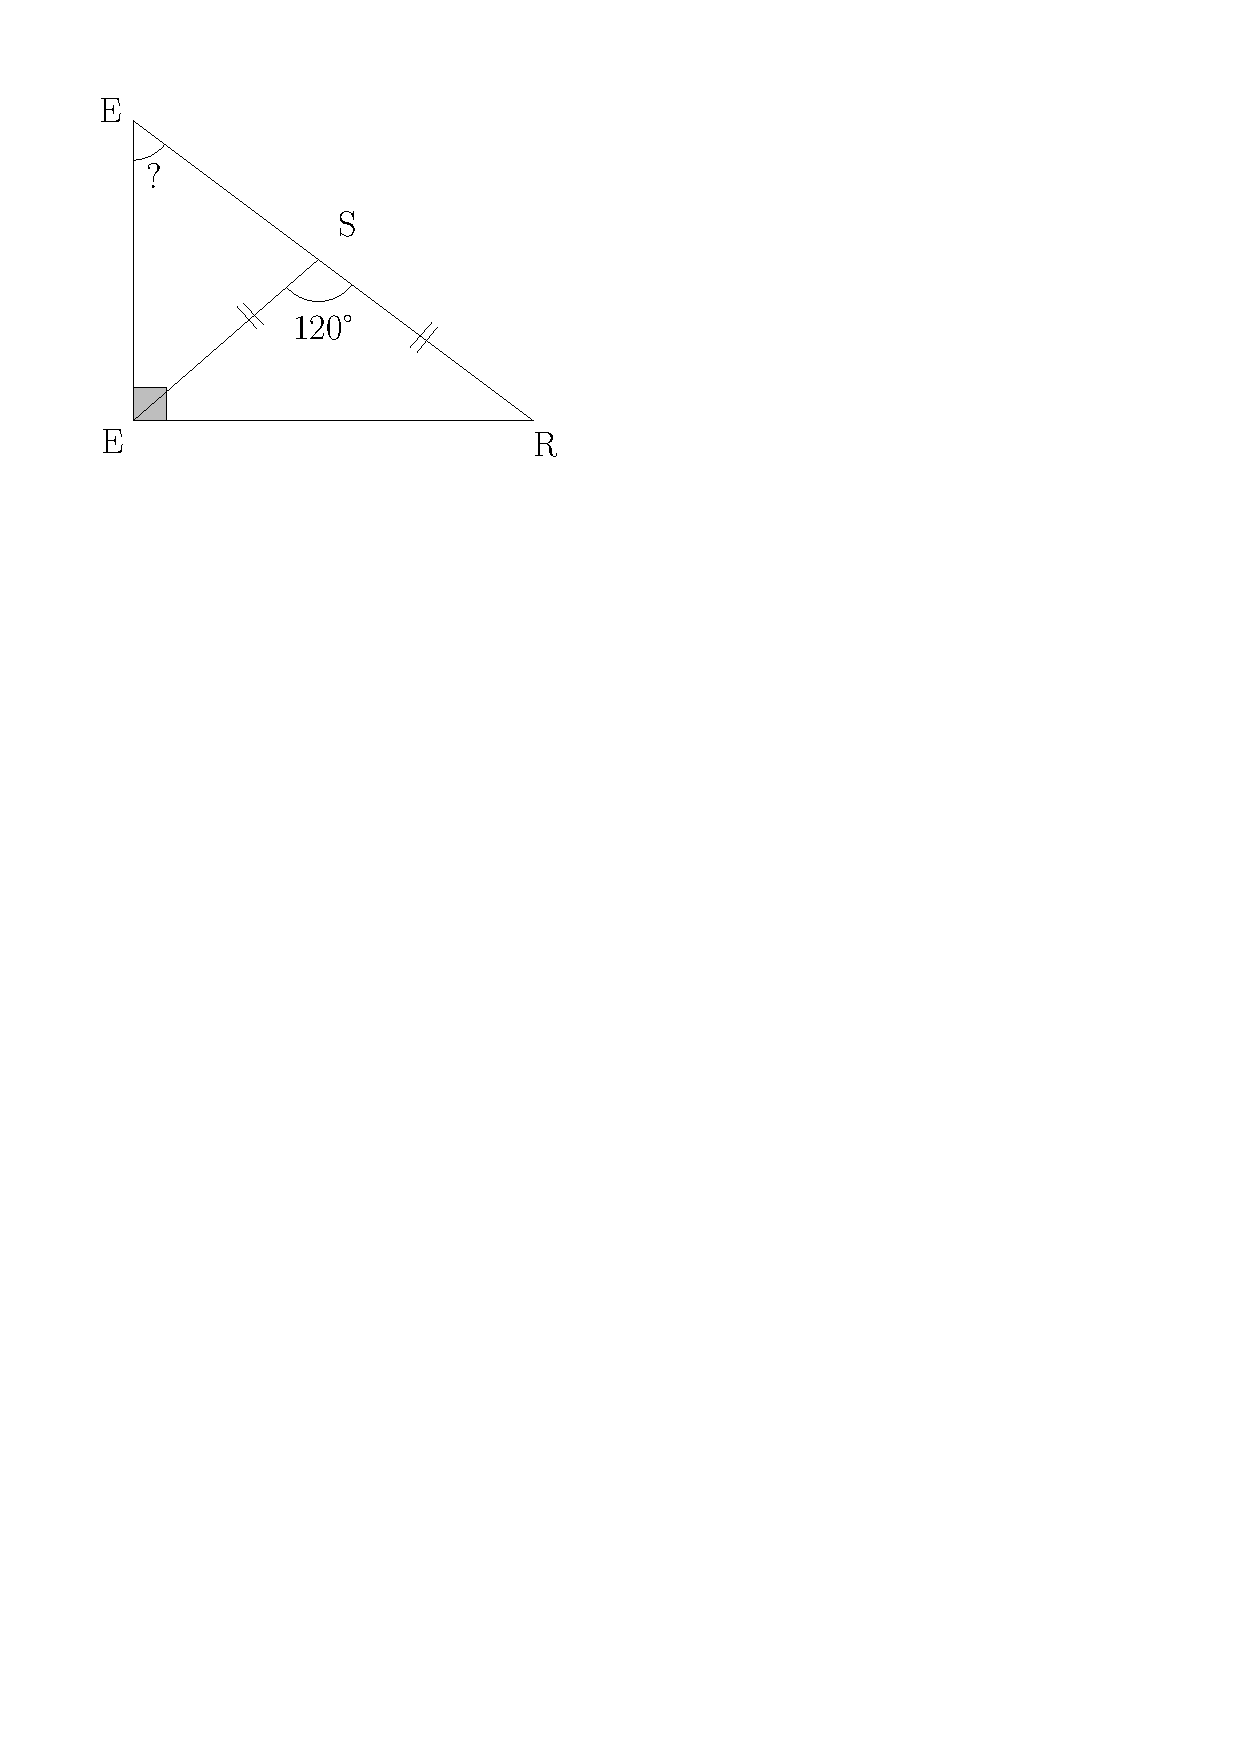
\includegraphics[width=0.6\linewidth]{5x3-triangles/ie-ex2a2.pdf}
  \end{figure}

\end{minipage}
\begin{minipage}[t]{0.6\textwidth}

  \Pointilles[8] \\
\end{minipage}

\begin{minipage}[t]{0.4\textwidth}
  \begin{figure}[H]
    \centering
    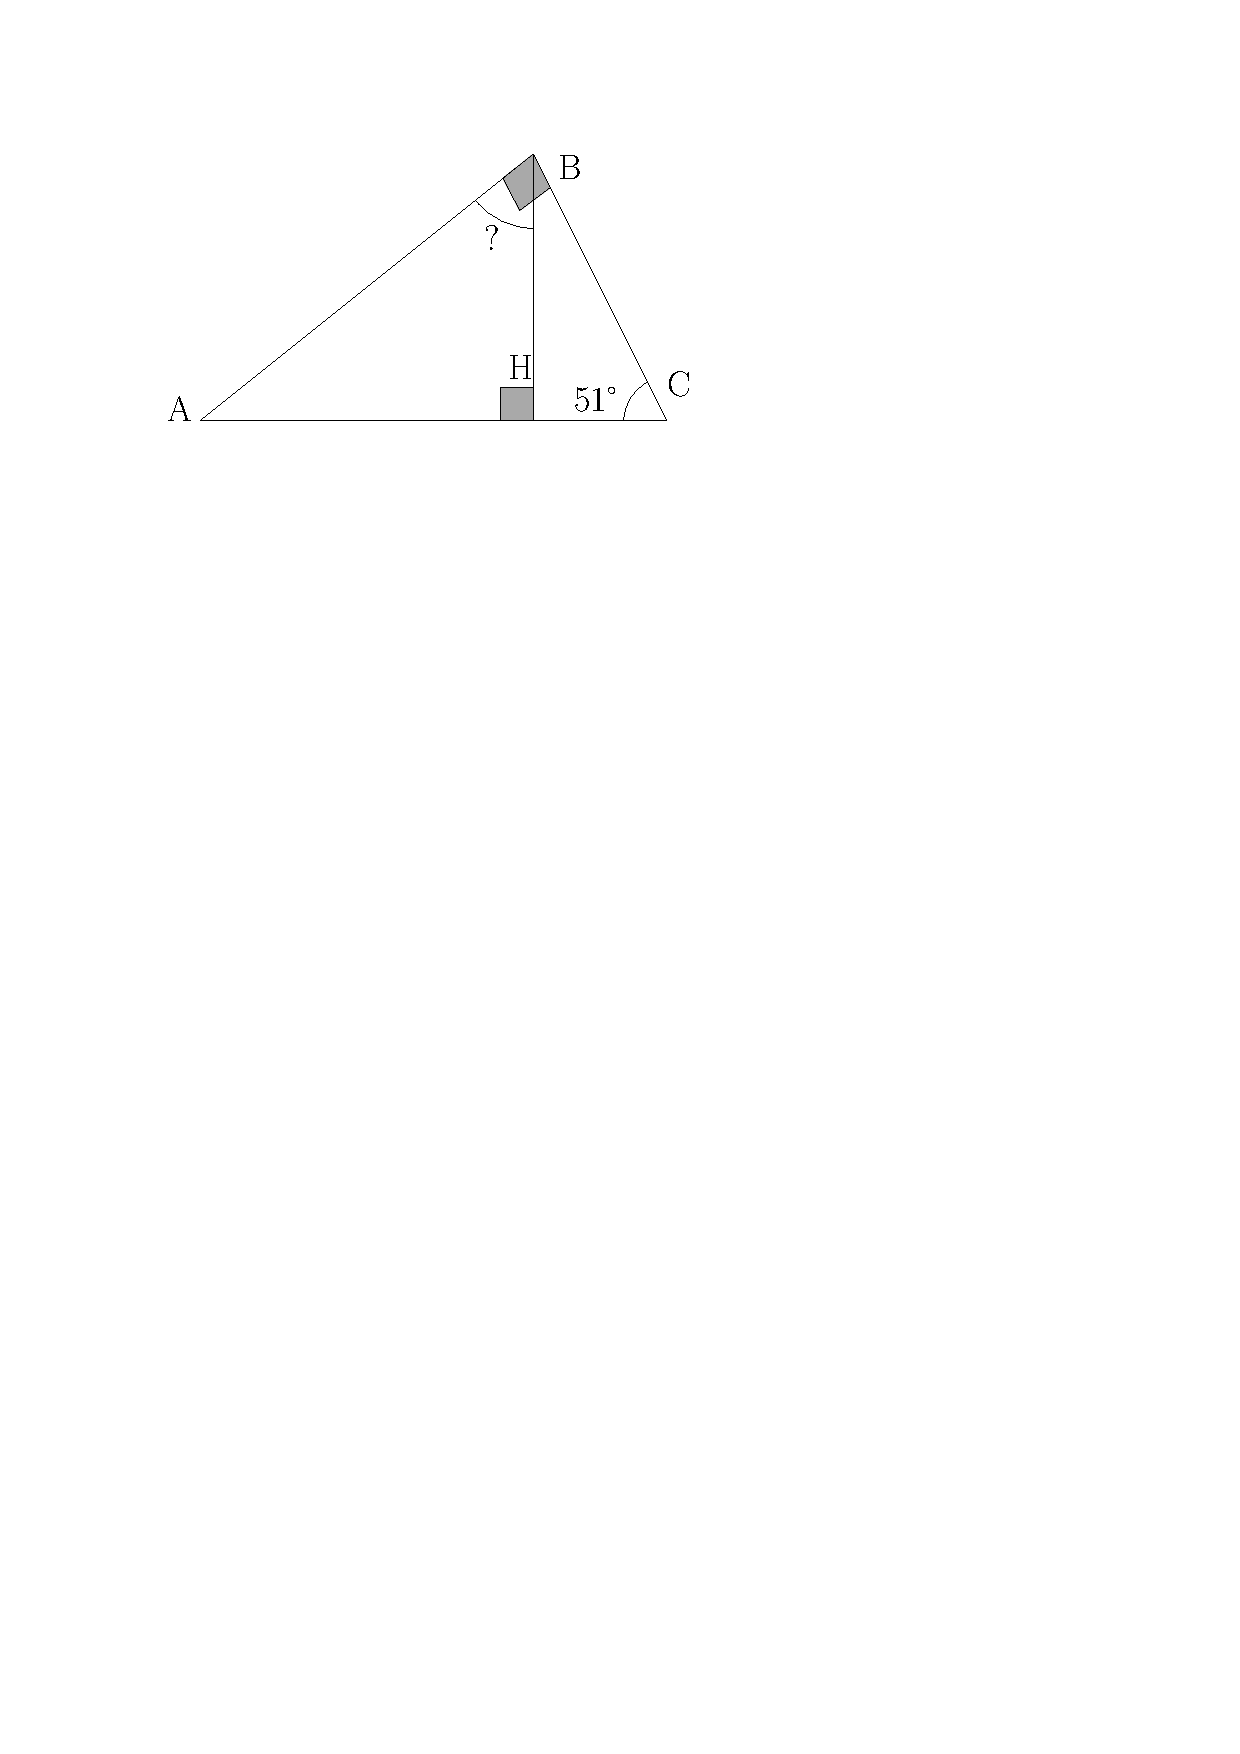
\includegraphics[width=0.8\linewidth]{5x3-triangles/ie-ex2b2.pdf}
  \end{figure} 

\end{minipage}
\begin{minipage}[t]{0.6\textwidth}

  \Pointilles[8] \\
\end{minipage}

\begin{minipage}[t]{0.4\textwidth}
\begin{figure}[H]
    \centering
    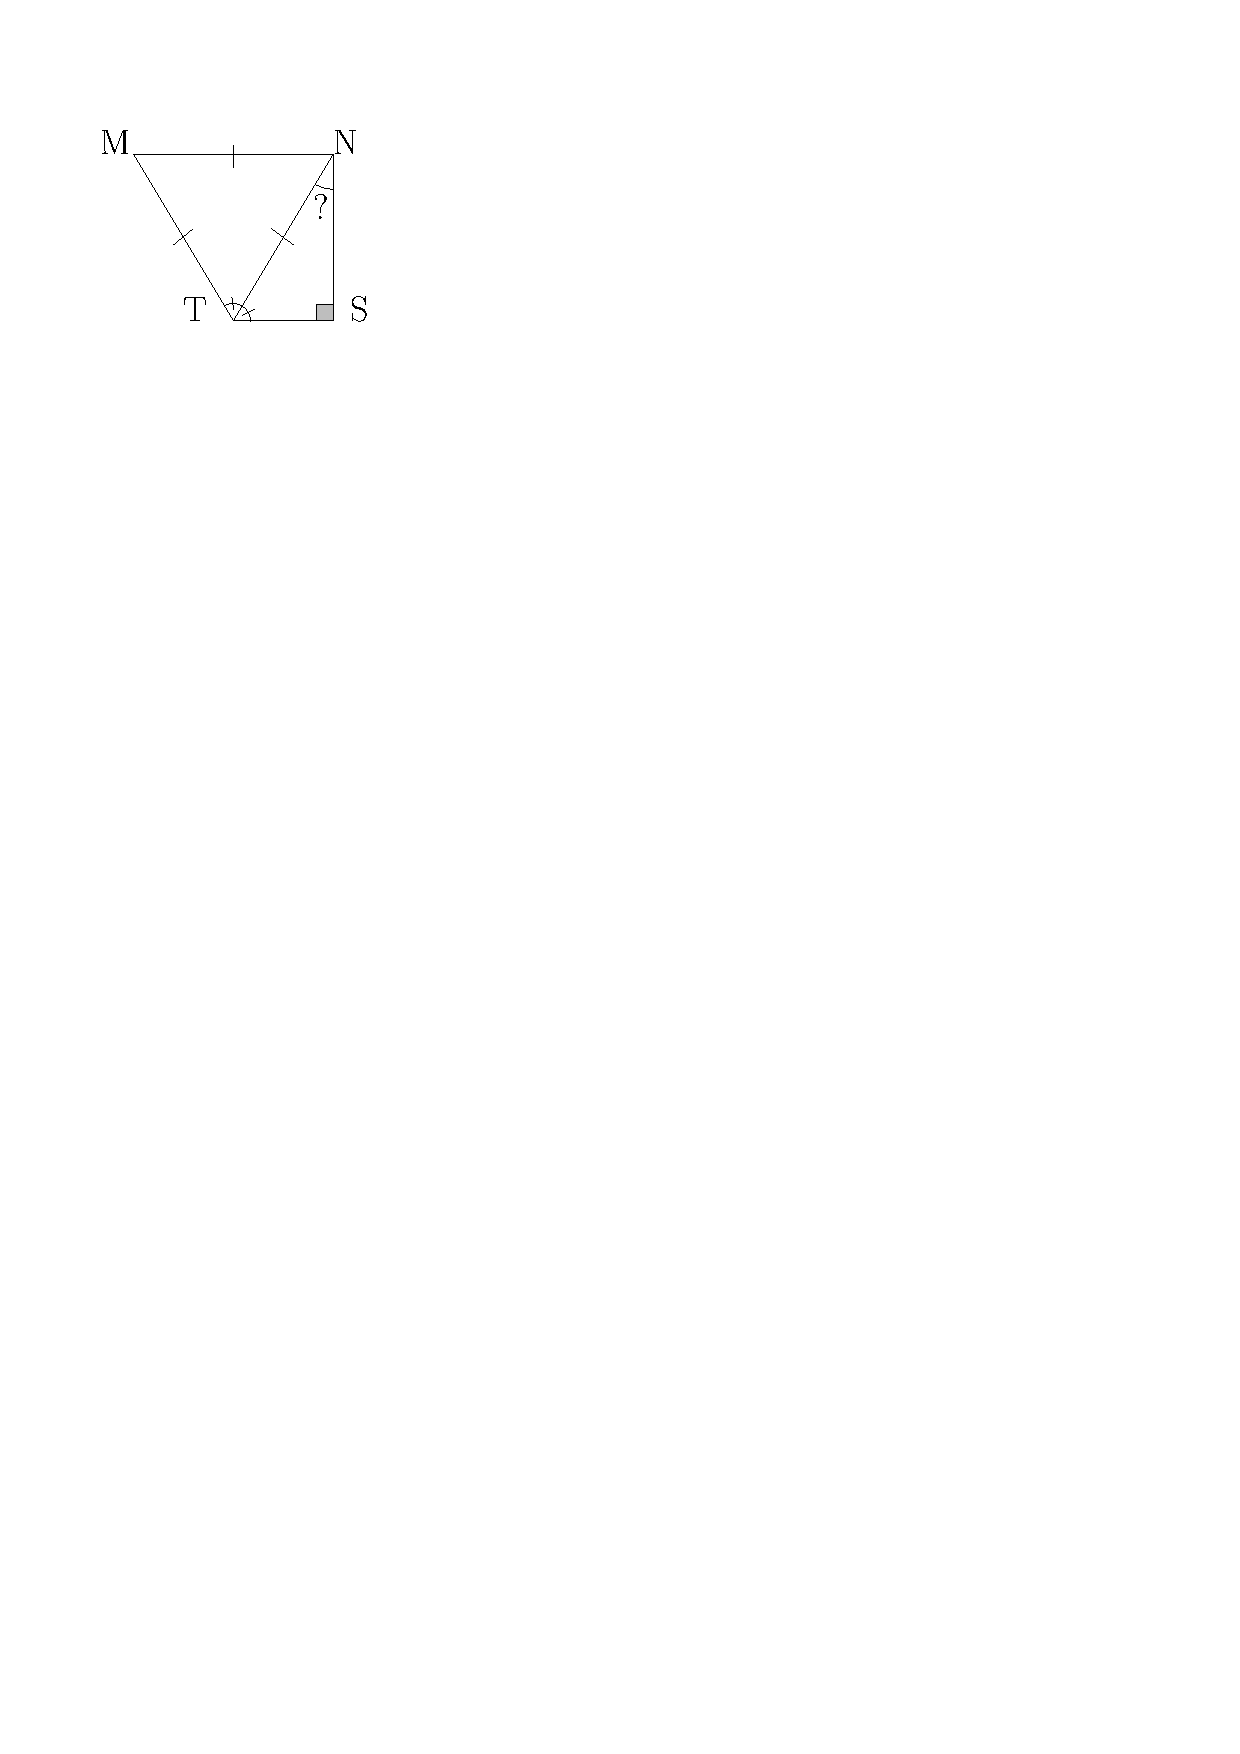
\includegraphics[width=0.6\linewidth]{5x3-triangles/ie-ex2c.pdf}
  \end{figure} 

\end{minipage}
\begin{minipage}[t]{0.6\textwidth}

  \Pointilles[8]
\end{minipage}



\subsection*{ex3 - Démontrer}

\begin{enumerate}
  \item[1.] \textbf{(aucune justification n'est demandée.)}

    Jean-mi veut construire un triangle ABC dont il connaît les longueurs AB et AC. \newline
    Parmi les longueurs proposées pour BC, \textbf{entourer la ou les mesures possibles}.

    \begin{multicols}{2}
      \begin{tabular}{|c|c||c|c|c|}
        \hline
          AB & AC & BC & BC & BC\\ \hline
          36 & 13 & 10 & 20 & 30\\ \hline
           6 & 10 & 10 & 20 & 30\\ \hline
          11 & 22 & 10 & 20 & 30\\ \hline
       $\pi$ & 16 & 10 & 20 & 30\\ \hline
      \end{tabular}
      
      \columnbreak

      \textit{(les pointillés peuvent servir de brouillon)}
      \Pointilles[4]
    \end{multicols}

  \item[2.] \textbf{(justifier, calculer, conclure.)}
  
  Soit ARN un triangle tel que AR = 14 cm et RN = 6 cm. \newline
  \textbf{Quelles sont les mesures entières possibles pour AN ?}

  \Pointilles[6]
\end{enumerate} 
\end{document}